% answers.tex —— 1977 年·辽宁卷 · 参考答案与详细解析片段
% 由 tools/generate_projects.py 依来源总账自 1977/1977_数学真题_辽宁_试题.md + 1977/1977_数学真题_辽宁_解析正文.md + 1977/1977_数学真题_辽宁_答案要点.md 生成，勿手改（改源 MD 后重跑）


\begin{gktip}
固定源是题面与解答连续出现的扫描材料。下文逐题独立推导并对照源解答复算关键结论；第 1 题大题号与小题编号的源卷体例及重排处理见试题卷题号说明；第 7 题源卷给出三种解法，本文按解法一思路推导并用余弦定理复核；参考题两题的解析接在第七题之后。
\end{gktip}

\begin{answer}
\gksolhead{1}{}

\textbf{题目}：

\begin{gktip}
\textbf{题号说明}：原卷第一题大题号未清晰印出（页首仅一残留短横），其下 5 个小题印作「1．」至「5．」；第 1 页两处附图题注印作「第一、4题附图」「第一，5题附图」，可证这 5 个小题同属第一大题。本库按规范重排为大题 1 与小问（1）至（5），未增删题干。
\end{gktip}

（1） 计算 $\sqrt{a^2-2ab+b^2}$（$a<b$）。

（2） 把 $x^5y-x^3y+2x^2y-xy$ 分解因式。

\Needspace{5\baselineskip}
（3） 计算：

\nopagebreak[4]
\[
\frac{0.027^{-\frac13}+\left(-\frac16\right)^{-2}-3^{-1}}{(-1000)^0-\operatorname{Log}_{10}\sqrt[3]{10}}\times 5^{\operatorname{Log}_5\frac23}.
\]

（4） 如图，$M$ 表示地平面，$PC$ 表示直立地面的电柱，$AC=6\,\mathrm{m}$，$BC$ 是 $AC$ 的 $\frac23$，求拉线 $AB$ 的长。（不必再写已知和求）

\begin{gktip}
原源 PDF 第 1 页附有地平面、电柱与拉线示意图（原卷题注「第一、4题附图」）；LaTeX 版按源图重绘。
\end{gktip}
\nopagebreak[4]
\begin{center}% 1977 年辽宁卷第一题(4)：地平面 M 上的电柱 PC，A 为拉线在柱上的锚固点（AC=6m），
% 拉线 AB 自 B 引至 A，BC 在地平面内（按源卷第 1 页「第一、4题附图」布局）
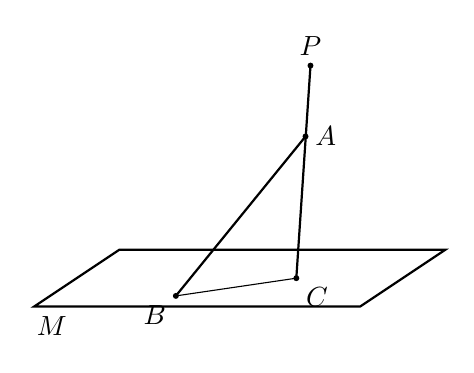
\begin{tikzpicture}[scale=0.9]
  % 地平面 M
  \draw[thick] (0,0) -- (4.6,0) -- (5.8,0.8) -- (1.2,0.8) -- cycle;
  \node[below] at (0.25,0) {$M$};
  % 电柱 PC：C 为柱脚，P 为柱顶，A 在 PC 上
  \draw[thick] (3.7,0.4) -- (3.9,3.4);
  \fill (3.9,3.4) circle (1.2pt) node[above] {$P$};
  \coordinate (A) at (3.83,2.4);
  \fill (A) circle (1.2pt) node[right] {$A$};
  \coordinate (C) at (3.7,0.4);
  \fill (C) circle (1.2pt) node[below right] {$C$};
  % 拉线 AB 与地面段 BC
  \draw[thick] (A) -- (2.0,0.15);
  \draw[thin] (C) -- (2.0,0.15);
  \fill (2.0,0.15) circle (1.2pt) node[below left] {$B$};
\end{tikzpicture}
\end{center}
\nopagebreak[4]
（5） 求出 $A(-3,3)$、$B(0,-1)$、$C(1,0)$ 三点中每两点间的距离，并指出以这三点为顶点的三角形 $ABC$ 是什么样的三角形。

\begin{gktip}
原源 PDF 第 1 页附有坐标系与三点示意图（原卷题注「第一，5题附图」）；LaTeX 版按源图重绘。
\end{gktip}
\nopagebreak[4]
\begin{center}% 1977 年辽宁卷第一题(5)：A(-3,3)、B(0,-1)、C(1,0) 三点与三角形 ABC（按源卷第 1 页「第一，5题附图」布局）
\begin{tikzpicture}[scale=0.72,>=stealth]
  \draw[->] (-4.2,0)--(5.4,0) node[below] {$x$};
  \draw[->] (0,-1.8)--(0,3.9) node[left] {$y$};
  \node[below left] at (0,0) {$O$};
  \draw[thin] (-3,0.07)--(-3,-0.07);
  \draw[thin] (1,0.07)--(1,-0.07);
  \draw[thin] (0.07,-1)--(-0.07,-1);
  \draw[thin] (0.07,3)--(-0.07,3);
  \draw[thick] (-3,3)--(0,-1)--(1,0)--cycle;
  \fill (-3,3) circle (1.2pt) node[left=2pt] {$A(-3,3)$};
  \fill (0,-1) circle (1.2pt) node[below right] {$B(0,-1)$};
  \fill (1,0) circle (1.2pt) node[above right] {$C(1,0)$};
\end{tikzpicture}
\end{center}
\nopagebreak[4]
\Needspace{4\baselineskip}
\textbf{解析}

\gksubpart{（1）}

\Needspace{5\baselineskip}
由 $a<b$ 知 $a-b<0$，负数的绝对值为其相反数，故

\nopagebreak[4]
\[
\sqrt{a^2-2ab+b^2}=\sqrt{(a-b)^2}=|a-b|=b-a.
\]

\gksubpart{（2）}

\nopagebreak[4]
\[
\begin{aligned}
x^5y-x^3y+2x^2y-xy
&=xy\left(x^4-x^2+2x-1\right)\\
&=xy\left[x^4-\left(x^2-2x+1\right)\right]\\
&=xy\left[x^4-(x-1)^2\right]\\
&=xy\left(x^2+x-1\right)\left(x^2-x+1\right).
\end{aligned}
\]

\gksubpart{（3）}

\Needspace{5\baselineskip}
各基本项的值：

\nopagebreak[4]
\[
0.027^{-\frac13}=\frac{10}{3},\qquad
\left(-\frac16\right)^{-2}=36,\qquad
3^{-1}=\frac13;
\]

\nopagebreak[4]
\[
(-1000)^0=1,\qquad
\operatorname{Log}_{10}\sqrt[3]{10}=\frac13,\qquad
5^{\operatorname{Log}_5\frac23}=\frac23.
\]

\Needspace{5\baselineskip}
于是

\nopagebreak[4]
\[
\begin{aligned}
\text{\text{原式}}
&=\frac{0.027^{-\frac13}+\left(-\frac16\right)^{-2}-3^{-1}}{(-1000)^0-\operatorname{Log}_{10}\sqrt[3]{10}}\times 5^{\operatorname{Log}_5\frac23}\\
&=\frac{\frac{10}{3}+36-\frac13}{1-\frac13}\times\frac23
=\frac{39}{\frac23}\times\frac23=39.
\end{aligned}
\]

\gksubpart{（4）}

\Needspace{5\baselineskip}
$PC$ 直立于地平面 $M$，即 $PC\perp M$，而 $BC$ 在平面 $M$ 内，故 $PC\perp BC$，$\angle ACB=90^\circ$，$\triangle ABC$ 为直角三角形。由 $BC$ 是 $AC$ 的 $\frac23$，

\nopagebreak[4]
\[
BC=\frac23\times6=4\ (\mathrm{m}).
\]

\Needspace{5\baselineskip}
由勾股定理，

\nopagebreak[4]
\[
AB=\sqrt{AC^2+BC^2}=\sqrt{6^2+4^2}=\sqrt{52}=2\sqrt{13}\ (\mathrm{m}).
\]

\gksubpart{（5）}

\Needspace{5\baselineskip}
由两点间距离公式，

\nopagebreak[4]
\[
\begin{aligned}
|AB|&=\sqrt{[0-(-3)]^2+(-1-3)^2}=\sqrt{9+16}=5,\\
|AC|&=\sqrt{[1-(-3)]^2+(0-3)^2}=\sqrt{16+9}=5,\\
|BC|&=\sqrt{(1-0)^2+[0-(-1)]^2}=\sqrt2.
\end{aligned}
\]

因为 $|AB|=|AC|$，所以 $\triangle ABC$ 是以 $A$ 为顶角的等腰三角形。

\gkanswer{答案（1）：$b-a$。}

\gkanswer{答案（2）：$xy(x^2+x-1)(x^2-x+1)$。}

\gkanswer{答案（3）：$39$。}

\gkanswer{答案（4）：$AB=2\sqrt{13}\ \mathrm{m}$。}

\gkanswer{答案（5）：$|AB|=|AC|=5$，$|BC|=\sqrt2$；$\triangle ABC$ 为等腰三角形。}

\end{answer}
\begin{answer}
\gksolhead{2}{}

\textbf{题目}：

判别二次函数 $y=x^2-4x+3$ 有最大值还是有最小值？并把它求出来；写出这个函数图象的顶点坐标，用描点法画出这个函数的图象。（画出草图即可）

\Needspace{4\baselineskip}
\textbf{解析}

\Needspace{5\baselineskip}
二次函数 $y=x^2-4x+3$ 的二次项系数 $a=1>0$，抛物线开口向上，函数有最小值。配方：

\nopagebreak[4]
\[
y=x^2-4x+3=(x-2)^2-1.
\]

当 $x=2$ 时函数取最小值 $-1$，顶点为 $(2,-1)$；对称轴 $x=2$，与 $x$ 轴交于 $(1,0)$、$(3,0)$，与 $y$ 轴交于 $(0,3)$。源卷解答按描点法列出：$x$ 取 $0\text{、}1\text{、}2$ 时，$y$ 依次为 $3\text{、}0\text{、}-1$。

图象草图：

\begin{gktip}
原源 PDF 第 2 页附有抛物线图象草图（原卷题注「第二题附图」）；LaTeX 版按源图重绘。
\end{gktip}
\nopagebreak[4]
\begin{center}% 1977 年辽宁卷第二题：y=x²-4x+3=(x-2)²-1 的图象草图，顶点 (2,-1)（按源卷第 2 页「第二题附图」布局）
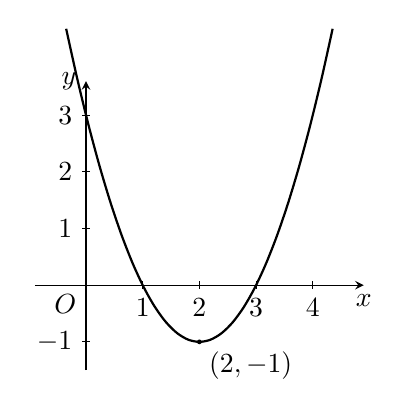
\begin{tikzpicture}[scale=0.72,>=stealth]
  \draw[->] (-0.9,0)--(4.9,0) node[below] {$x$};
  \draw[->] (0,-1.5)--(0,3.6) node[left] {$y$};
  \node[below left] at (0,0) {$O$};
  \foreach \x in {1,2,3,4}{
    \draw[thin] (\x,0.07)--(\x,-0.07) node[below] {$\x$};
  }
  \foreach \y in {-1,1,2,3}{
    \draw[thin] (0.07,\y)--(-0.07,\y) node[left] {$\y$};
  }
  \draw[thick,domain=-0.35:4.35,smooth] plot (\x,{\x*\x-4*\x+3});
  \fill (2,-1) circle (1.2pt);
  \node[below right] at (2,-1) {$(2,-1)$};
\end{tikzpicture}
\end{center}
\nopagebreak[4]
\gkanswer{答案：有最小值。当 $x=2$ 时最小值 $-1$，顶点 $(2,-1)$；图象草图见解析版。}

\end{answer}
\begin{answer}
\gksolhead{3}{}

\textbf{题目}：

制造某种产品，计划经过两年使成本降低 36\%，问平均每年应降低百分之几？

\Needspace{4\baselineskip}
\textbf{解析}

\Needspace{5\baselineskip}
设原来成本为 $1$，平均每年应降低的百分数为 $x$。经过两年后成本为 $(1-x)^2$，由题意

\nopagebreak[4]
\[
(1-x)^2=1-36\%=0.64,
\]

\nopagebreak[4]
\[
1-x=\pm0.8,
\qquad
x=0.2\ \text{\text{或}}\ x=1.8.
\]

$x=1.8$ 即 $180\%$，降低幅度超过全部成本，不合题意，舍去。所以平均每年应降低 $20\%$。

\gkanswer{答案：$20\%$。}

\end{answer}
\begin{answer}
\gksolhead{4}{}

\textbf{题目}：

在 $\triangle ABC$ 中，已知 $\operatorname{Cos}A=\dfrac5{13}$，$\operatorname{Cos}B=\dfrac35$，求 $\operatorname{Cos}C$ 的值。

\Needspace{4\baselineskip}
\textbf{解析}

\Needspace{5\baselineskip}
因为 $A+B+C=180^\circ$，所以

\nopagebreak[4]
\[
\begin{aligned}
\operatorname{Cos}C
&=\operatorname{Cos}\left[180^\circ-(A+B)\right]
=-\operatorname{Cos}(A+B)\\
&=\operatorname{Sin}A\cdot\operatorname{Sin}B-\operatorname{Cos}A\cdot\operatorname{Cos}B.
\end{aligned}
\]

\Needspace{5\baselineskip}
由 $A\text{、}B$ 为三角形内角，$\operatorname{Sin}A\text{、}\operatorname{Sin}B>0$，

\nopagebreak[4]
\[
\operatorname{Sin}A=\sqrt{1-\operatorname{Cos}^2A}
=\sqrt{1-\left(\frac5{13}\right)^2}=\frac{12}{13},
\]

\nopagebreak[4]
\[
\operatorname{Sin}B=\sqrt{1-\operatorname{Cos}^2B}
=\sqrt{1-\left(\frac35\right)^2}=\frac45.
\]

\Needspace{5\baselineskip}
代入，得

\nopagebreak[4]
\[
\operatorname{Cos}C=\frac{12}{13}\cdot\frac45-\frac5{13}\cdot\frac35
=\frac{48}{65}-\frac{15}{65}=\frac{33}{65}.
\]

\gkanswer{答案：$\dfrac{33}{65}$。}

\end{answer}
\begin{answer}
\gksolhead{5}{}

\textbf{题目}：

求证：两条对角线相等的梯形是等腰梯形（画出图形，写出：已知、求证、证明）。

\Needspace{4\baselineskip}
\textbf{解析}

按题面要求写出已知、求证并证明。

已知：四边形 $ABCD$ 是梯形，$DC\parallel AB$，$AC$ 和 $BD$ 是对角线，且 $AC=BD$。

求证：$AD=BC$。

\textbf{证法一}

作 $CE\perp AB$，垂足为 $E$；作 $DF\perp AB$，垂足为 $F$。

\begin{gktip}
原源 PDF 第 3 页附有梯形与两条垂线示意图（原卷题注「第五题证法一附图」）；LaTeX 版按源图重绘。
\end{gktip}
\nopagebreak[4]
\begin{center}% 1977 年辽宁卷第五题证法一：梯形 ABCD（DC∥AB），CE⊥AB 于 E、DF⊥AB 于 F（按源卷第 3 页「第五题证法一附图」布局）
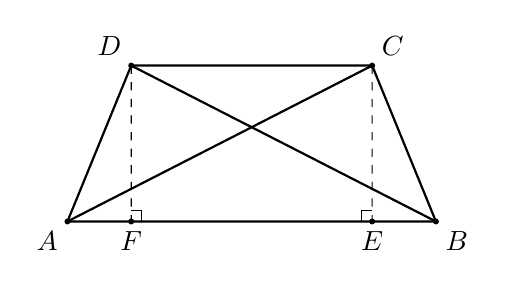
\begin{tikzpicture}[scale=0.9]
  \coordinate (A) at (0,0);
  \coordinate (B) at (5.2,0);
  \coordinate (D) at (0.9,2.2);
  \coordinate (C) at (4.3,2.2);
  \draw[thick] (A)--(B)--(C)--(D)--cycle;
  \draw[thick] (A)--(C);
  \draw[thick] (B)--(D);
  \draw[dashed] (C)--(4.3,0);
  \draw[dashed] (D)--(0.9,0);
  \fill (A) circle (1.2pt) node[below left] {$A$};
  \fill (B) circle (1.2pt) node[below right] {$B$};
  \fill (D) circle (1.2pt) node[above left] {$D$};
  \fill (C) circle (1.2pt) node[above right] {$C$};
  \fill (4.3,0) circle (1.2pt) node[below] {$E$};
  \fill (0.9,0) circle (1.2pt) node[below] {$F$};
  % 直角标记
  \draw[thin] (4.15,0) -- (4.15,0.15) -- (4.3,0.15);
  \draw[thin] (1.05,0) -- (1.05,0.15) -- (0.9,0.15);
\end{tikzpicture}
\end{center}
\nopagebreak[4]
\Needspace{5\baselineskip}
因为 $DC\parallel AB$，$CE$ 与 $DF$ 都是两平行线间的垂线段，所以

\nopagebreak[4]
\[
CE=DF.
\]

\Needspace{5\baselineskip}
在直角三角形 $ACE$ 和 $BDF$ 中，$CE=DF$，$AC=BD$，由斜边直角边定理，

\nopagebreak[4]
\[
\mathrm{Rt}\triangle ACE\cong\mathrm{Rt}\triangle BDF,
\]

\Needspace{5\baselineskip}
所以

\nopagebreak[4]
\[
\angle CAE=\angle DBF.
\]

\Needspace{5\baselineskip}
即在 $\triangle CAB$ 与 $\triangle DBA$ 中，$AC=BD$，$\angle CAB=\angle DBA$，$AB=AB$（公用边），由边角边定理，

\nopagebreak[4]
\[
\triangle CAB\cong\triangle DBA,
\]

\Needspace{5\baselineskip}
所以

\nopagebreak[4]
\[
AD=BC.
\]

\textbf{证法二}

作 $CE\parallel DB$，交 $AB$ 的延长线于 $E$；又 $DC\parallel BE$，所以四边形 $DBEC$ 是平行四边形。

\begin{gktip}
原源 PDF 第 3 页附有梯形与辅助线 $CE$ 示意图（原卷题注「第五题证法二附图」）；LaTeX 版按源图重绘。
\end{gktip}
\nopagebreak[4]
\begin{center}% 1977 年辽宁卷第五题证法二：作 CE∥DB 交 AB 的延长线于 E，DBEC 为平行四边形
% （按源卷第 3 页「第五题证法二附图」布局；E 在 B 右侧，CE 与 DB 平行，BE 为延长线虚线）
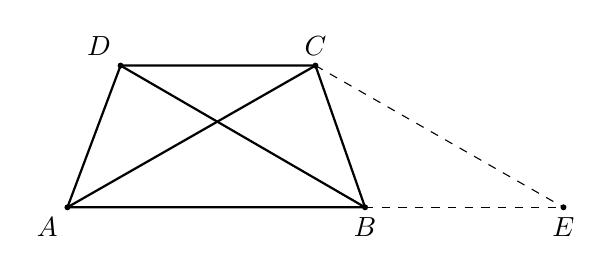
\begin{tikzpicture}[scale=0.9]
  \coordinate (A) at (0,0);
  \coordinate (B) at (4.2,0);
  \coordinate (D) at (0.75,2.0);
  \coordinate (C) at (3.5,2.0);
  \coordinate (E) at (7.0,0);
  \draw[thick] (A)--(B)--(C)--(D)--cycle;
  \draw[thick] (A)--(C);
  \draw[thick] (B)--(D);
  \draw[dashed] (C)--(E);
  \draw[dashed] (B)--(E);
  \fill (A) circle (1.2pt) node[below left] {$A$};
  \fill (B) circle (1.2pt) node[below] {$B$};
  \fill (D) circle (1.2pt) node[above left] {$D$};
  \fill (C) circle (1.2pt) node[above] {$C$};
  \fill (E) circle (1.2pt) node[below] {$E$};
\end{tikzpicture}
\end{center}
\nopagebreak[4]
\Needspace{5\baselineskip}
由平行四边形对边相等，

\nopagebreak[4]
\[
EC=BD.
\]

\Needspace{5\baselineskip}
又 $AC=BD$，所以 $AC=EC$，从而

\nopagebreak[4]
\[
\angle CAB=\angle CEA.
\]

\Needspace{5\baselineskip}
又 $DB\parallel CE$，同位角相等，

\nopagebreak[4]
\[
\angle DBA=\angle CEA,
\]

\Needspace{5\baselineskip}
所以 $\angle CAB=\angle DBA$。在 $\triangle DAB$ 和 $\triangle CBA$ 中，$DB=AC$，$\angle DBA=\angle CAB$，$AB=AB$，由边角边定理，

\nopagebreak[4]
\[
\triangle DAB\cong\triangle CBA,
\]

\Needspace{5\baselineskip}
所以

\nopagebreak[4]
\[
AD=BC.
\]

\textbf{证法三}

设 $AC$、$BD$ 交于 $O$ 点。

\begin{gktip}
原源 PDF 第 4 页附有梯形对角线交于 $O$ 及内错角标记示意图（原卷题注「第五题 证法三附图」）；LaTeX 版按源图重绘。
\end{gktip}
\nopagebreak[4]
\begin{center}% 1977 年辽宁卷第五题证法三：对角线 AC、BD 交于 O，∠1=∠2、∠3=∠4（内错角）
% （按源卷第 4 页「第五题 证法三附图」布局）
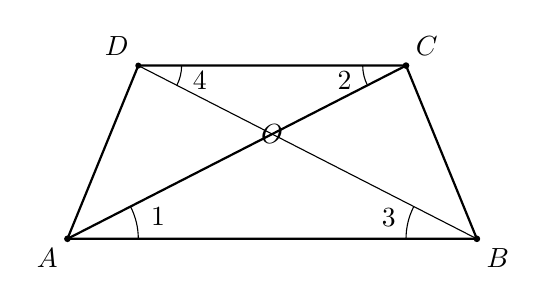
\begin{tikzpicture}[scale=1.0]
  \coordinate (A) at (0,0);
  \coordinate (B) at (5.2,0);
  \coordinate (D) at (0.9,2.2);
  \coordinate (C) at (4.3,2.2);
  \draw[thick] (A)--(B)--(C)--(D)--cycle;
  \draw[thick] (A)--(C);
  \draw[thin] (B)--(D);
  \draw[thin] ([shift={(A)}]0:0.9) arc[start angle=0,end angle=27.1,radius=0.9];
  \draw[thin] ([shift={(C)}]180:0.55) arc[start angle=180,end angle=207.1,radius=0.55];
  \draw[thin] ([shift={(B)}]152.9:0.9) arc[start angle=152.9,end angle=180,radius=0.9];
  \draw[thin] ([shift={(D)}]-27.1:0.55) arc[start angle=-27.1,end angle=0,radius=0.55];
  \node at (1.15,0.28) {$1$};
  \node at (3.52,2.01) {$2$};
  \node at (4.08,0.27) {$3$};
  \node at (1.68,2.01) {$4$};
  \node at (2.60,1.33) {$O$};
  \fill (A) circle (1.2pt) node[below left] {$A$};
  \fill (B) circle (1.2pt) node[below right] {$B$};
  \fill (D) circle (1.1pt) node[above left] {$D$};
  \fill (C) circle (1.2pt) node[above right] {$C$};
\end{tikzpicture}
\end{center}
\nopagebreak[4]
\Needspace{5\baselineskip}
因为 $DC\parallel AB$，内错角相等，

\nopagebreak[4]
\[
\angle1=\angle2,\qquad
\angle3=\angle4.
\]

\Needspace{5\baselineskip}
所以 $\triangle AOB\sim\triangle COD$，对应边成比例，

\nopagebreak[4]
\[
\frac{AO}{OC}=\frac{BO}{OD}.
\]

\Needspace{5\baselineskip}
因此

\nopagebreak[4]
\[
\frac{AO+OC}{OC}=\frac{BO+OD}{OD},
\]

\Needspace{5\baselineskip}
即

\nopagebreak[4]
\[
\frac{AC}{OC}=\frac{BD}{OD}.
\]

\Needspace{5\baselineskip}
由 $AC=BD$，得

\nopagebreak[4]
\[
OC=OD.
\]

\Needspace{5\baselineskip}
所以 $\angle2=\angle4$（等边对等角）。在 $\triangle ADC$ 和 $\triangle BCD$ 中，$AC=BD$，$\angle2=\angle4$，$DC=DC$（公用边），由边角边定理，

\nopagebreak[4]
\[
\triangle ADC\cong\triangle BCD,
\]

\Needspace{5\baselineskip}
所以

\nopagebreak[4]
\[
AD=BC.
\]

\gkanswer{答案：见解析版}

\end{answer}
\begin{answer}
\gksolhead{6}{}

\textbf{题目}：

$\alpha$ 是多少度时，方程 $2x^2+2\sqrt2\,x+\operatorname{tg}\alpha=0$ 有两个相等的实数根？（$0^\circ\le\alpha<360^\circ$）

\Needspace{4\baselineskip}
\textbf{解析}

\Needspace{5\baselineskip}
一元二次方程 $2x^2+2\sqrt2\,x+\operatorname{tg}\alpha=0$ 有两个相等的实数根，须判别式为零。这里二次项系数 $a=2$，一次项系数 $b=2\sqrt2$，常数项 $c=\operatorname{tg}\alpha$：

\nopagebreak[4]
\[
b^2-4ac=(2\sqrt2)^2-4\times2\times\operatorname{tg}\alpha
=8-8\operatorname{tg}\alpha=0.
\]

\Needspace{5\baselineskip}
所以

\nopagebreak[4]
\[
\operatorname{tg}\alpha=1.
\]

\Needspace{5\baselineskip}
又 $0^\circ\le\alpha<360^\circ$，正切值为 $1$ 的角在此范围内有两个，

\nopagebreak[4]
\[
\alpha=45^\circ\ \text{\text{或}}\ \alpha=225^\circ.
\]

即 $\alpha=45^\circ$ 或 $\alpha=225^\circ$ 时，方程有两个相等的实数根。

\gkanswer{答案：$\alpha=45^\circ$ 或 $\alpha=225^\circ$。}

\end{answer}
\begin{answer}
\gksolhead{7}{}

\textbf{题目}：

如图，我海军某舰艇在 $A$ 处测得入侵敌舰在方位角为 $45^\circ$、距离为 10 海里的 $C$ 处，并正沿方位角为 $105^\circ$ 的方向以每小时 9 海里的速度逃跑，我舰艇立即以每小时 21 海里的速度沿直线前去追捕，问我舰艇应沿多大的方位角和需用多少小时才能在某处 $B$ 追上敌舰？

（已知：$\operatorname{Sin}21^\circ47'=\dfrac{3\sqrt3}{14}$，$\operatorname{Sin}38^\circ13'=\dfrac{5\sqrt3}{14}$。这两个数据可根据解题需要取用。）

\begin{gktip}
原源 PDF 第 4 页附有 A、C 两处北向箭头与追击路线示意图（原卷题注「第七题附图」）；LaTeX 版按源图重绘。
\end{gktip}
\nopagebreak[4]
\begin{center}% 1977 年辽宁卷第七题：A 处测得敌舰 C（方位角 45°、距离 10 海里），
% 敌舰沿方位角 105° 方向逃跑，我舰沿海面直线 AB 追至 B 追上
% （按源卷第 4 页「第七题附图」布局：A、C 处各画北向箭头，A 处标 45°，C 处标 105°）
\begin{tikzpicture}[scale=0.62,>=stealth]
  \coordinate (A) at (0,0);
  \coordinate (C) at (3.5,3.5);
  \coordinate (B) at (9.3,1.95);
  \draw[->] (A) -- (0,2.2) node[draw=none,above] {北};
  \draw[->] (C) -- (3.5,5.2) node[draw=none,above] {北};
  \draw[thick] (A)--(B)--(C)--cycle;
  \draw[thin] ([shift={(A)}]45:0.8) arc[start angle=45,end angle=90,radius=0.8];
  \node at (0.40,0.97) {$45^\circ$};
  \draw[thin] ([shift={(C)}]-15:0.7) arc[start angle=-15,end angle=90,radius=0.7];
  \node at (4.25,4.08) {$105^\circ$};
  \fill (A) circle (1.2pt) node[below left] {$A$};
  \fill (C) circle (1.2pt) node[above left] {$C$};
  \fill (B) circle (1.2pt) node[right] {$B$};
\end{tikzpicture}
\end{center}
\nopagebreak[4]
\begin{gktip}
\textbf{参考题}
\end{gktip}

\textbf{参考题 1．} 某生产队要建造一个已知体积为 $V$ 的有盖圆柱形氨水池，问这个氨水池的高 $h$ 和底面半径 $r$ 取多大时，用料最省？

\begin{gktip}
原源 PDF 第 7 页附有氨水池（圆柱）高 $h$ 与底面半径 $r$ 示意图；LaTeX 版按源图重绘。
\end{gktip}
\nopagebreak[4]
\begin{center}% 1977 年辽宁卷参考题一：有盖圆柱形氨水池，标高 h 与底面半径 r（按源卷第 7 页布局）
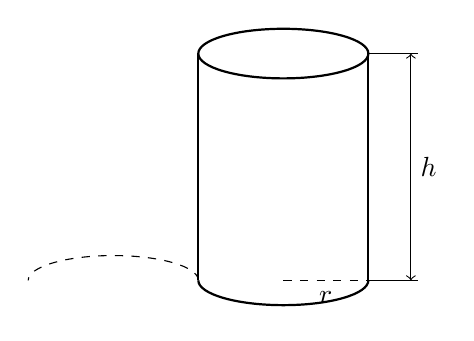
\begin{tikzpicture}[scale=0.9]
  \draw[thick] (1.2,3.2) ellipse (1.2 and 0.35);
  \draw[thick] (0,3.2)--(0,0);
  \draw[thick] (2.4,3.2)--(2.4,0);
  \draw[thick] (0,0) arc[x radius=1.2,y radius=0.35,start angle=180,end angle=360];
  \draw[dashed] (0,0) arc[x radius=1.2,y radius=0.35,start angle=0,end angle=180];
  % 底面半径 r（中心到右缘，虚线）
  \draw[dashed] (1.2,0)--(2.4,0);
  \node[draw=none,below] at (1.8,-0.02) {$r$};
  % 高 h（右侧尺寸线）
  \draw[thin] (2.4,0) -- (3.1,0);
  \draw[thin] (2.4,3.2) -- (3.1,3.2);
  \draw[<->] (3.0,0)--(3.0,3.2) node[midway,right] {$h$};
\end{tikzpicture}
\end{center}
\nopagebreak[4]
\textbf{参考题 2．} 求 $y=\operatorname{Sin}x$（$x$ 在 $[0,\pi]$ 上）与 $x$ 轴所围成的图形的面积。
\nopagebreak[4]
\begin{center}% 1977 年辽宁卷参考题二：y=Sinx 在 [0,π] 与 x 轴之间的阴影区域（按源卷第 7 页「参考题二附图」布局）
% 源卷图内标注印作「y=Sinπ」，系排印之误，重绘图按 y=Sinx 标注
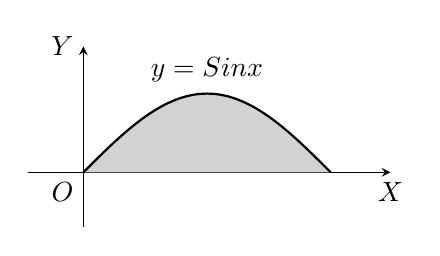
\begin{tikzpicture}[scale=1.0,>=stealth]
  \draw[->] (-0.7,0)--(3.9,0) node[below] {$X$};
  \draw[->] (0,-0.7)--(0,1.6) node[left] {$Y$};
  \node[below left] at (0,0) {$O$};
  \fill[gray!35] (0,0) -- plot[domain=0:3.1416,smooth] (\x,{sin(\x r)}) -- cycle;
  \draw[thick,domain=0:3.1416,smooth] plot (\x,{sin(\x r)});
  \node[draw=none,above] at (1.57,1.02) {$y=\operatorname{Sin}x$};
\end{tikzpicture}
\end{center}
\nopagebreak[4]
\begin{gktip}
原源 PDF 第 7 页附有 $y=\operatorname{Sin}x$ 在 $[0,\pi]$ 上与 $x$ 轴之间的阴影区域示意图（源卷图内标注印作「y=Sinπ」，系排印之误）；LaTeX 版按源图重绘并按 $y=\operatorname{Sin}x$ 标注。
\end{gktip}

\Needspace{4\baselineskip}
\textbf{解析}
\nopagebreak[4]
\begin{center}% 1977 年辽宁卷第七题：A 处测得敌舰 C（方位角 45°、距离 10 海里），
% 敌舰沿方位角 105° 方向逃跑，我舰沿海面直线 AB 追至 B 追上
% （按源卷第 4 页「第七题附图」布局：A、C 处各画北向箭头，A 处标 45°，C 处标 105°）
\begin{tikzpicture}[scale=0.62,>=stealth]
  \coordinate (A) at (0,0);
  \coordinate (C) at (3.5,3.5);
  \coordinate (B) at (9.3,1.95);
  \draw[->] (A) -- (0,2.2) node[draw=none,above] {北};
  \draw[->] (C) -- (3.5,5.2) node[draw=none,above] {北};
  \draw[thick] (A)--(B)--(C)--cycle;
  \draw[thin] ([shift={(A)}]45:0.8) arc[start angle=45,end angle=90,radius=0.8];
  \node at (0.40,0.97) {$45^\circ$};
  \draw[thin] ([shift={(C)}]-15:0.7) arc[start angle=-15,end angle=90,radius=0.7];
  \node at (4.25,4.08) {$105^\circ$};
  \fill (A) circle (1.2pt) node[below left] {$A$};
  \fill (C) circle (1.2pt) node[above left] {$C$};
  \fill (B) circle (1.2pt) node[right] {$B$};
\end{tikzpicture}
\end{center}
\nopagebreak[4]
\Needspace{5\baselineskip}
设我舰艇在某处 $B$ 追上敌舰需用 $x$ 小时，则在 $\triangle ABC$ 中，

\nopagebreak[4]
\[
AB=21x,\qquad BC=9x\ (\text{\text{海里}}),\qquad AC=10\ (\text{\text{海里}}).
\]

\Needspace{5\baselineskip}
求 $\angle C$：$A$ 看 $C$ 的方位角是 $45^\circ$，反过来 $C$ 看 $A$ 的方位角是 $225^\circ$；敌舰逃跑方向的方位角是 $105^\circ$，故

\nopagebreak[4]
\[
\angle C=225^\circ-105^\circ=120^\circ.
\]

\Needspace{5\baselineskip}
由正弦定理，

\nopagebreak[4]
\[
\frac{21x}{\operatorname{Sin}120^\circ}=\frac{9x}{\operatorname{Sin}A},
\]

\Needspace{5\baselineskip}
所以

\nopagebreak[4]
\[
\operatorname{Sin}A=\frac{9x}{21x}\operatorname{Sin}120^\circ
=\frac37\operatorname{Sin}60^\circ=\frac{3\sqrt3}{14}.
\]

\Needspace{5\baselineskip}
又 $\angle C=120^\circ$，故 $A$ 必为锐角，而

\nopagebreak[4]
\[
\operatorname{Sin}21^\circ47'=\frac{3\sqrt3}{14},
\]

\Needspace{5\baselineskip}
所以

\nopagebreak[4]
\[
\angle A=21^\circ47'.
\]

\Needspace{5\baselineskip}
我舰艇新航向的方位角是在原 $45^\circ$ 基础上再转过度数 $21^\circ47'$：

\nopagebreak[4]
\[
45^\circ+21^\circ47'=66^\circ47'.
\]

\Needspace{5\baselineskip}
三角形内角和给出

\nopagebreak[4]
\[
\angle B=180^\circ-120^\circ-21^\circ47'=38^\circ13'.
\]

\Needspace{5\baselineskip}
再由正弦定理求 $x$：

\nopagebreak[4]
\[
\frac{9x}{\operatorname{Sin}21^\circ47'}=\frac{10}{\operatorname{Sin}38^\circ13'},
\]

\nopagebreak[4]
\[
x=\frac{10\operatorname{Sin}21^\circ47'}{9\operatorname{Sin}38^\circ13'}
=\frac{10\cdot\frac{3\sqrt3}{14}}{9\cdot\frac{5\sqrt3}{14}}
=\frac{30}{45}=\frac23\ (\text{\text{小时}}).
\]

即追上敌舰需 $\frac23$ 小时，合 40 分钟。

\Needspace{5\baselineskip}
\textbf{余弦定理复核}：在 $\triangle ABC$ 中，

\nopagebreak[4]
\[
(21x)^2=10^2+(9x)^2-2\cdot10\cdot(9x)\operatorname{Cos}120^\circ.
\]

\Needspace{5\baselineskip}
整理，得

\nopagebreak[4]
\[
360x^2-9x-10=0,
\]

\Needspace{5\baselineskip}
解得

\nopagebreak[4]
\[
x_1=\frac23,\qquad
x_2=-\frac5{12}\ (\text{\text{不合题意，舍去}}).
\]

$x=\frac23$ 与正弦定理所得一致，且此时 $AB=21x=14$ 海里、$BC=9x=6$ 海里，与 $\angle A=21^\circ47'$（$\operatorname{Cos}A=\frac{13}{14}$）互洽。

\begin{gktip}
\textbf{源注}：源卷对本题给出正弦定理、正弦余弦联用、余弦定理三种解法，结论均为方位角 $66^\circ47'$、用时 $\frac23$ 小时；本文以正弦定理解答、余弦定理复核。
\end{gktip}

\textbf{参考题 1}
\nopagebreak[4]
\begin{center}% 1977 年辽宁卷参考题一：有盖圆柱形氨水池，标高 h 与底面半径 r（按源卷第 7 页布局）
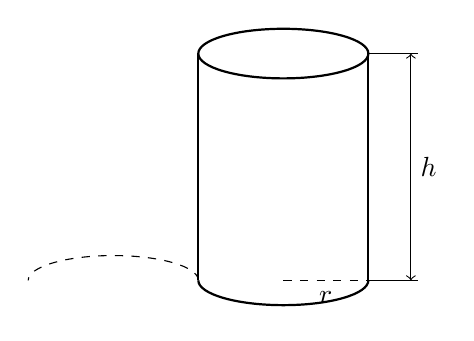
\begin{tikzpicture}[scale=0.9]
  \draw[thick] (1.2,3.2) ellipse (1.2 and 0.35);
  \draw[thick] (0,3.2)--(0,0);
  \draw[thick] (2.4,3.2)--(2.4,0);
  \draw[thick] (0,0) arc[x radius=1.2,y radius=0.35,start angle=180,end angle=360];
  \draw[dashed] (0,0) arc[x radius=1.2,y radius=0.35,start angle=0,end angle=180];
  % 底面半径 r（中心到右缘，虚线）
  \draw[dashed] (1.2,0)--(2.4,0);
  \node[draw=none,below] at (1.8,-0.02) {$r$};
  % 高 h（右侧尺寸线）
  \draw[thin] (2.4,0) -- (3.1,0);
  \draw[thin] (2.4,3.2) -- (3.1,3.2);
  \draw[<->] (3.0,0)--(3.0,3.2) node[midway,right] {$h$};
\end{tikzpicture}
\end{center}
\nopagebreak[4]
\Needspace{5\baselineskip}
用料最省即氨水池的表面积最小。设表面积为 $S$，有盖圆柱的表面积为上、下两底面与侧面之和：

\nopagebreak[4]
\[
S=2\pi r^2+2\pi rh.
\]

\Needspace{5\baselineskip}
由体积为 $V$，

\nopagebreak[4]
\[
V=\pi r^2h,
\qquad
h=\frac{V}{\pi r^2}.
\]

\Needspace{5\baselineskip}
代入表面积式，便得到 $S$ 为 $r$ 的函数：

\nopagebreak[4]
\[
S=S(r)=2\pi r^2+\frac{2V}{r}.
\]

\Needspace{5\baselineskip}
下面讨论 $r$ 取什么值时 $S$ 最小。求导：

\nopagebreak[4]
\[
S'(r)=4\pi r-\frac{2V}{r^2}.
\]

\Needspace{5\baselineskip}
令 $S'(r)=0$，即

\nopagebreak[4]
\[
4\pi r-\frac{2V}{r^2}=0
\quad\Longrightarrow\quad
r^3=\frac{V}{2\pi},
\]

\Needspace{5\baselineskip}
方程只有一个实数根

\nopagebreak[4]
\[
r=\sqrt[3]{\frac{V}{2\pi}}
=\frac{\sqrt[3]{4\pi^2V}}{2\pi}.
\]

\Needspace{5\baselineskip}
从这个实际问题知道表面积应有最小值，所以 $r$ 取该值时 $S$ 最小。这时相应的高为

\nopagebreak[4]
\[
h=\frac{V}{\pi r^2}=\frac{2\pi r^3}{\pi r^2}=2r
=\frac{\sqrt[3]{4\pi^2V}}{\pi}.
\]

即高和底面直径相等时，用料最省。

\textbf{参考题 2}
\nopagebreak[4]
\begin{center}% 1977 年辽宁卷参考题二：y=Sinx 在 [0,π] 与 x 轴之间的阴影区域（按源卷第 7 页「参考题二附图」布局）
% 源卷图内标注印作「y=Sinπ」，系排印之误，重绘图按 y=Sinx 标注
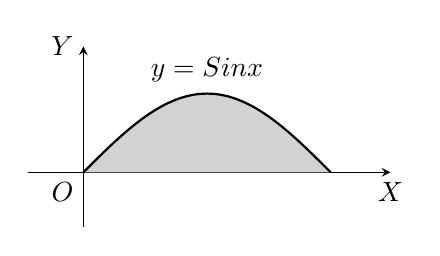
\begin{tikzpicture}[scale=1.0,>=stealth]
  \draw[->] (-0.7,0)--(3.9,0) node[below] {$X$};
  \draw[->] (0,-0.7)--(0,1.6) node[left] {$Y$};
  \node[below left] at (0,0) {$O$};
  \fill[gray!35] (0,0) -- plot[domain=0:3.1416,smooth] (\x,{sin(\x r)}) -- cycle;
  \draw[thick,domain=0:3.1416,smooth] plot (\x,{sin(\x r)});
  \node[draw=none,above] at (1.57,1.02) {$y=\operatorname{Sin}x$};
\end{tikzpicture}
\end{center}
\nopagebreak[4]
\Needspace{5\baselineskip}
因为 $x$ 在 $[0,\pi]$ 上，$\operatorname{Sin}x\ge0$，所以所求图形的面积是

\nopagebreak[4]
\[
S=\int_0^{\pi}\operatorname{Sin}x\,dx.
\]

\Needspace{5\baselineskip}
由积分基本公式，

\nopagebreak[4]
\[
\begin{aligned}
S
&=\left(-\operatorname{Cos}x\right)\Big|_0^{\pi}\\
&=-\operatorname{Cos}\pi-\left(-\operatorname{Cos}0\right)\\
&=1-(-1)=2.
\end{aligned}
\]

\gkanswer{答案：应沿方位角 $66^\circ47'$ 前去追捕，需 $\dfrac23$ 小时（即 40 分钟）。}

\end{answer}